\documentclass[tikz,border=8pt]{standalone}
\usepackage{amsmath,amssymb}
\usetikzlibrary{arrows.meta,automata,positioning,quotes}
\begin{document}
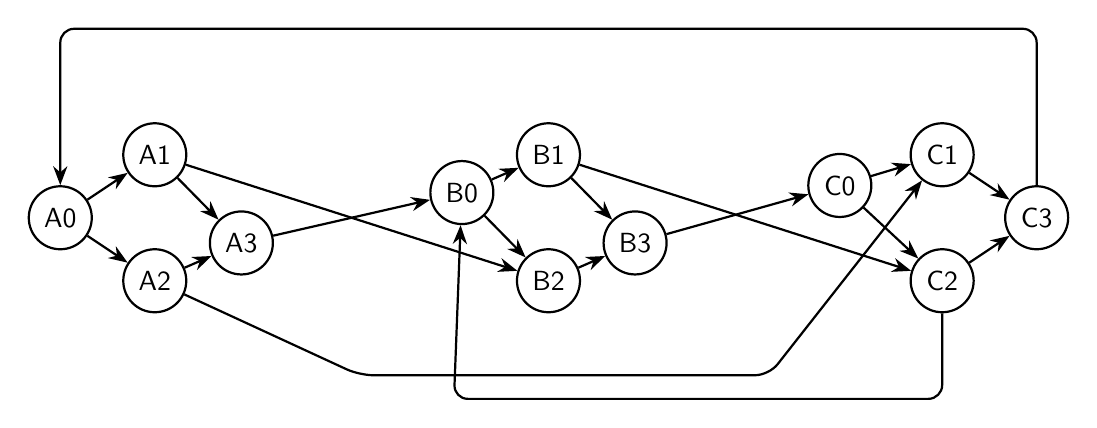
\begin{tikzpicture}[x=1cm,y=1cm]
\tikzset{
  graphnode/.style={circle,draw,thick,minimum size=8mm,inner sep=1pt,font=\sffamily},
  directed/.style={-{Stealth[length=2.4mm]},thick},
  undirected/.style={thick}
}
\node[graphnode] (n_A0) at (0.00,0.00) {A0};
\node[graphnode] (n_A1) at (1.20,0.80) {A1};
\node[graphnode] (n_A2) at (1.20,-0.80) {A2};
\node[graphnode] (n_A3) at (2.30,-0.32) {A3};
\node[graphnode] (n_B0) at (5.10,0.32) {B0};
\node[graphnode] (n_B1) at (6.20,0.80) {B1};
\node[graphnode] (n_B2) at (6.20,-0.80) {B2};
\node[graphnode] (n_B3) at (7.30,-0.32) {B3};
\node[graphnode] (n_C0) at (9.90,0.41) {C0};
\node[graphnode] (n_C1) at (11.20,0.80) {C1};
\node[graphnode] (n_C2) at (11.20,-0.80) {C2};
\node[graphnode] (n_C3) at (12.40,0.00) {C3};
\draw[directed] (n_A0) -- (n_A1);
\draw[directed] (n_A0) -- (n_A2);
\draw[directed] (n_A1) -- (n_A3);
\draw[directed] (n_A2) -- (n_A3);
\draw[directed] (n_B0) -- (n_B1);
\draw[directed] (n_B0) -- (n_B2);
\draw[directed] (n_B1) -- (n_B3);
\draw[directed] (n_B2) -- (n_B3);
\draw[directed] (n_C0) -- (n_C1);
\draw[directed] (n_C0) -- (n_C2);
\draw[directed] (n_C1) -- (n_C3);
\draw[directed] (n_C2) -- (n_C3);
\draw[directed] (n_A3) -- (n_B0);
\draw[directed] (n_B3) -- (n_C0);
\draw[directed] (n_A1) -- (n_B2);
\draw[directed,rounded corners=5pt] (n_A2) -- (3.80,-2.00) -- (9.00,-2.00) -- (n_C1);
\draw[directed] (n_B1) -- (n_C2);
\draw[directed,rounded corners=5pt] (n_C3) -- (12.40,2.40) -- (0.00,2.40) -- (n_A0);
\draw[directed,rounded corners=5pt] (n_C2) -- (11.20,-2.30) -- (5.00,-2.30) -- (n_B0);
\end{tikzpicture}
\end{document}
